\documentclass[letterpaper, margin=1in]{article}

\usepackage[english]{babel}
\usepackage[utf8]{inputenc}
\usepackage{amsmath}
\usepackage{graphicx}
\usepackage[colorinlistoftodos]{todonotes}
\usepackage{geometry}
\def\MLine#1{\par\hspace*{-\leftmargin}\parbox{\textwidth}{\[#1\]}}

\title{Crime and Punishment | final project for CAPP 30255}

\author{Carlos Grandet and Hector Salvador}

\date{\today}

\begin{document}
\maketitle

\begin{abstract}
We made a first version of a question-answering program that retrieves a set of potential answers to questions like: What is the penalty for committing murder?. We use the 300 current Mexican federal laws, specifically attempting to retrieve criminal and administrative sentences (e.g. jail years, fines, political disablement). We implement this machine in Python, using the framework described by Jurafsky and Martin \cite{jurafsky}. We show our results, challenges, and potential next steps to improve our machine.

\textbf{Keywords:} question-answering machine, natural language processing, Mexican federal laws, text analysis.
\end{abstract}

\section{Introduction}
\label{sec:introduction}

We thought a question answering machine was a good idea for a final project because:
\begin{itemize}
\item This could empower people to look if certain sentences or penalties are real. In a corrupt country like Mexico, sometimes people don't know if the punishment they're receiving is even legally sound. A lot of people would not dare to contradict a judge or a lawyer, just because they don't have any education to understand laws. 
\item It's hard to read lots of laws at once. Hector worked in the past with regulations in energy and had to quickly understand 14 new laws when they came out. This took him a very long time to read, especially since laws sometimes use a particular language and understanding them correctly takes a lot of time.
\item Since we're Mexican, we wanted to do a text analysis project in Spanish. We were very happy to  be able to apply many of the concepts we learned in class: dynamic programming, word2vec, n-gram models with Hidden Markov Models, and information retrieval (IR).
\end{itemize}


\section{Framework}
\label{sec:theory}

\subsection{Overview}

We followed the three stages of an IR-based factoid question answering machine (figure 	\ref{fig:pipeline}). We scraped 300 Mexican federal laws from the Mexican congress website\footnote{http://www.diputados.gob.mx/LeyesBiblio/index.htm}. We then used these documents to create passages (a smaller unit of documents) that would be retrieved by an IR algorithm. Finally, we prioritize these passages, using a combination of BM25 and the probability of the passage containing an answer. Because of time constraints (we had less than 1/3 of a 10-week quarter to work on this project), we could not do any work on the answer processing part of the pipeline.

\begin{figure}
\centering
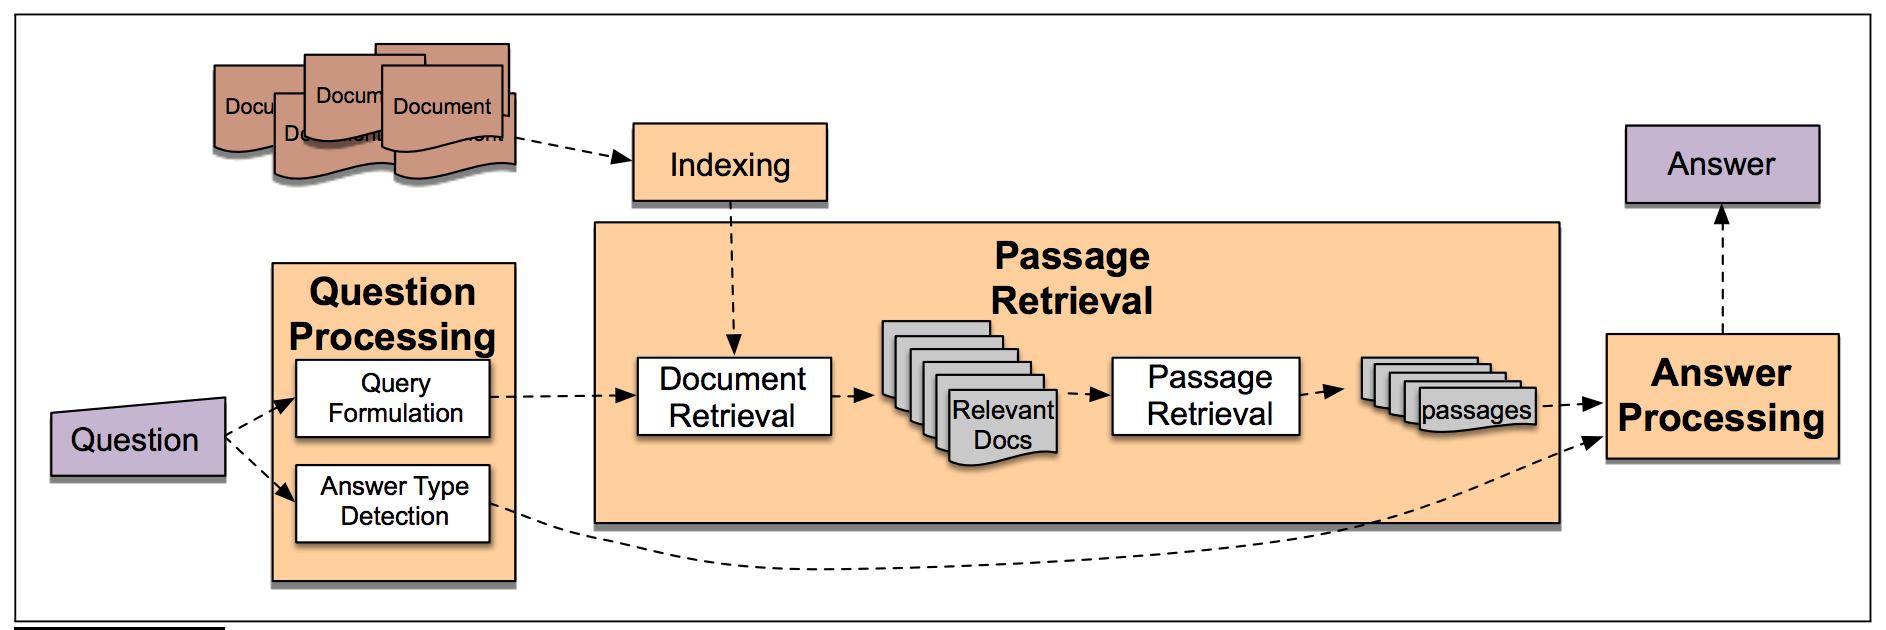
\includegraphics[width=1\textwidth]{pipeline.png}
\caption{\label{fig:pipeline}IR-based factoid question answering has three stages: question processing, passage retrieval, and answer processing. This is Figure 28.2 from \cite{jurafsky}, Chapter 28.1.1.}
\end{figure}

\subsection{Document creation}
Scraping was done using \texttt{scrape.py}. Laws were available both in \texttt{pdf} and \texttt{doc} files. Two methods were tested to convert the files to \texttt{txt} files that could be processed in Python. 

First we tried converting \texttt{pdf} files to \texttt{txt} using out-of-the-box packages (e.g. using \texttt{pdftotext} utility in the command line). Unfortunately, Mexican laws have a ton of useless text as headers and footnotes \ref{fig:header}, which are repeated over all documents. This introduced a lot of noise in our models, so we tried next using \texttt{doc} files.

We attempted unsuccessfully to just open \texttt{doc} files in Python. There were a lot of binary characters that made reading and text processing difficult. Maybe it was our lack of experience opening files, but we could not find a way to retrieve only the text we needed, especially since many characters have accents in Spanish. We also tried using \texttt{antiword} and \texttt{python-docx}, but we kept having installation errors, even using a virtual environment\footnote{Using a macOS Sierra 10.12.3 and python 3.5}.

After spending several hours, we opted to manually convert \texttt{doc} files to \texttt{txt} manually. These can all be found in the folder called \texttt{/leyes/*}.

\begin{figure}
\centering

\includegraphics[width=1\textwidth]{header.png}
\caption{\label{fig:header}Example of the top part of a Mexican Law saved as a doc file. Notice the headers, the titles, subtitles, and additional text that is non-informative.}
\end{figure}

\subsection{Question processing}
Explain the IQHE in your own words. What does the density of states look like in a 2-DEG when $B=0$? What are Landau levels and how do they arise? What are edge states? What does the electron transport look like when you change the magnetic field? What do you expect to measure?

\subsection{Document retrieval}


\subsection{What didn't work?}

\section{Results}
\subsection{Why}
Explain a step-by-step recipe for fabrication here. How long did you etch and why? What is an Ohmic contact?

\newpage
\section{How to run the code}

\subsection{Dependencies}
\begin{itemize}
\item requests, bs4, for the scraping
\item synonyms
\item gensim 
\item nltk, for stem.snowball.SpanishStemmer, tokenize.RegexpTokenizer
\item textblob, for easy word manipulation
\item jellyfish, for Jaro-Winkler sitance
\item sklearn, for general processing, including TF, IDF, and Multinomial Naive Bayes models
\item numpy, pandas
\end{itemize}

\subsection{Instructions}
Before running the code, make sure that the \texttt{txt} files are in folder called leyes and that the file called \texttt{docnames.csv} is in the folder called \texttt{doc}.

\begin{enumerate}
\item Open a Python shell, preferably ipython.
\item If you want to download the \texttt{doc} files, run \\ \texttt{\$ run scrape.py} \\ then call \\ \texttt{\$ go()} \\ This will download the \texttt{doc} files in the folder called \texttt{/doc}.
\item Open a Python shell, preferably ipython.
\end{enumerate}

Alternatively, you can use the \texttt{jupyter notebook} titled \texttt{QA{\_}machine}, available in the root directory of the repository.

\begin{thebibliography}{9}
\bibitem{jurafsky}
  Jurafsky, Dan, and James H. Martin. 
  \emph{Speech and language processing: an introduction to natural language processing, computational linguistics, and speech recognition.} 
  India: Dorling Kindersley Pvt, Ltd., 2014.

\end{thebibliography}

\newpage
\appendix

\section{Repository structure}
The repository has the following folders:
\begin{itemize}
\item \texttt{Data}
\item \texttt{doc}
\item \texttt{indices}
\item \texttt{leyes}
\item \texttt{stanford-postagger-full-2016-10-31}
\end{itemize}

It also has a bunch of Python scripts and miscellaneous files:

\begin{itemize}
\item \texttt{scrape.py}
\item \texttt{index.py}
\item \texttt{ngrams.py}
\item \texttt{query.py}
\item \texttt{question{\_}processing.py}
\item \texttt{retrieval.py}
\item \texttt{spanish{\_}tagger.py}
\item \texttt{synonyms.py}
\item \texttt{Word2VecModel.py}
\end{itemize}

Miscellaneous:
\begin{itemize}
\item \texttt{get{\_}l.sh}: count average document length to use in BM25 algorithm.
\end{itemize}

\end{document}